\documentclass{article}

\usepackage[T1]{fontenc}
\usepackage[utf8]{inputenc}
\usepackage[french]{babel}
\usepackage[affil-it]{authblk}
\usepackage{fullpage}
\usepackage{graphicx}
\usepackage{biblatex}
\usepackage{stackengine}
\usepackage{listings}

\newenvironment*{remerciements}{%
  \renewcommand*{\abstractname}{Remerciements}
  \begin{abstract}
}{
  \end{abstract}
}

\bibliography{introduction/sources}
\bibliography{centralisation/sources}
\bibliography{decentralisation/sources}


\begin{document}

\title{Echange de jetons inter-blockchains}
\author{VOLPE Dorian, ROTONDO Eloïse, TESTUD Romain,\\DE CAMPOU Louis, JOLY Amaury  \\ \textbf{Encadrants :} TRAVERS Corentin, LABOUREL Arnaud \\ 
\includegraphics[scale=0.1]{./img/amu.png}}
\affil{Aix-Marseille Université, M2 Fiabilité et sécurité informatique}
\date{17 Mars 2023}

\begin{titlepage}
  \maketitle
\end{titlepage}

\begin{remerciements}
  Merci à M. TRAVERS Corentin et M. LABOUREL Arnaud pour la proposition de ce sujet et son encadrement.
\end{remerciements}
\begin{abstract}
  abstract
\end{abstract}

\newpage

\tableofcontents

\newpage

\section{Introduction}
\begin{frame}{Centralisé}
    \begin{block}{Le centralisé offre\dots}
        \begin{itemize}
            \item Diversité d'acteurs.
            \item Accessibilité.
            \item Multiples fonctionnalités.
        \end{itemize}
    \end{block}
    \pause
    \begin{block}{Mais\dots}
        \begin{itemize}
            \item Opacité des protocoles.
            \item Failles de sécurité.
            \item Collecte des données.
        \end{itemize}
    \end{block}
\end{frame}


\begin{frame}{Décentralisé}
    \begin{block}{Le décentralisé offre\dots\dots}
        \begin{itemize}
            \item Pas de tiers de confiance.
            \item Transparence.
            \item Fiabilité accrue.
        \end{itemize}
    \end{block}
    \pause
    \begin{block}{Mais\dots}
        \begin{itemize}
            \item Difficiles d'accès.
            \item Intérêt économique faible.
        \end{itemize}
    \end{block}
\end{frame}

\begin{frame}{Conclusion générale}
    \begin{itemize}
        \item Flou entre centralisé/décentralisé.
        \item Définition variable.
    \end{itemize}
\end{frame}

\begin{frame}
    \begin{figure}
        \begin{figure}
            \centering
            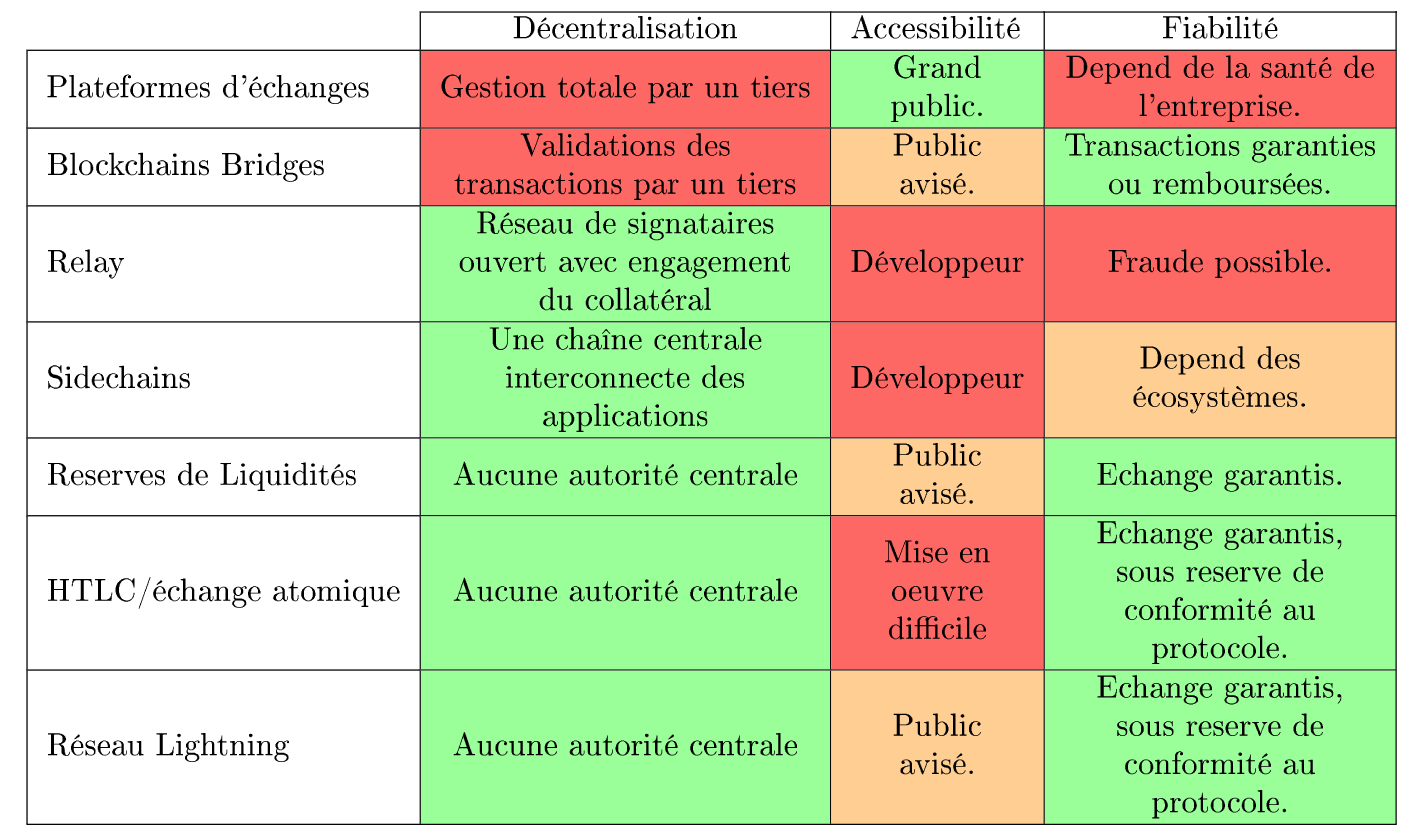
\includegraphics[scale = 0.2]{conclusion/tableau.png}
            \label{fig:recap}
            \caption{Tableau récapitulatif}
        \end{figure}
    \end{figure}
    
\end{frame}

\newpage
\section{Systèmes Centralisés}
\begin{frame}{Centralisé}
    \begin{block}{Le centralisé offre\dots}
        \begin{itemize}
            \item Diversité d'acteurs.
            \item Accessibilité.
            \item Multiples fonctionnalités.
        \end{itemize}
    \end{block}
    \pause
    \begin{block}{Mais\dots}
        \begin{itemize}
            \item Opacité des protocoles.
            \item Failles de sécurité.
            \item Collecte des données.
        \end{itemize}
    \end{block}
\end{frame}


\begin{frame}{Décentralisé}
    \begin{block}{Le décentralisé offre\dots\dots}
        \begin{itemize}
            \item Pas de tiers de confiance.
            \item Transparence.
            \item Fiabilité accrue.
        \end{itemize}
    \end{block}
    \pause
    \begin{block}{Mais\dots}
        \begin{itemize}
            \item Difficiles d'accès.
            \item Intérêt économique faible.
        \end{itemize}
    \end{block}
\end{frame}

\begin{frame}{Conclusion générale}
    \begin{itemize}
        \item Flou entre centralisé/décentralisé.
        \item Définition variable.
    \end{itemize}
\end{frame}

\begin{frame}
    \begin{figure}
        \begin{figure}
            \centering
            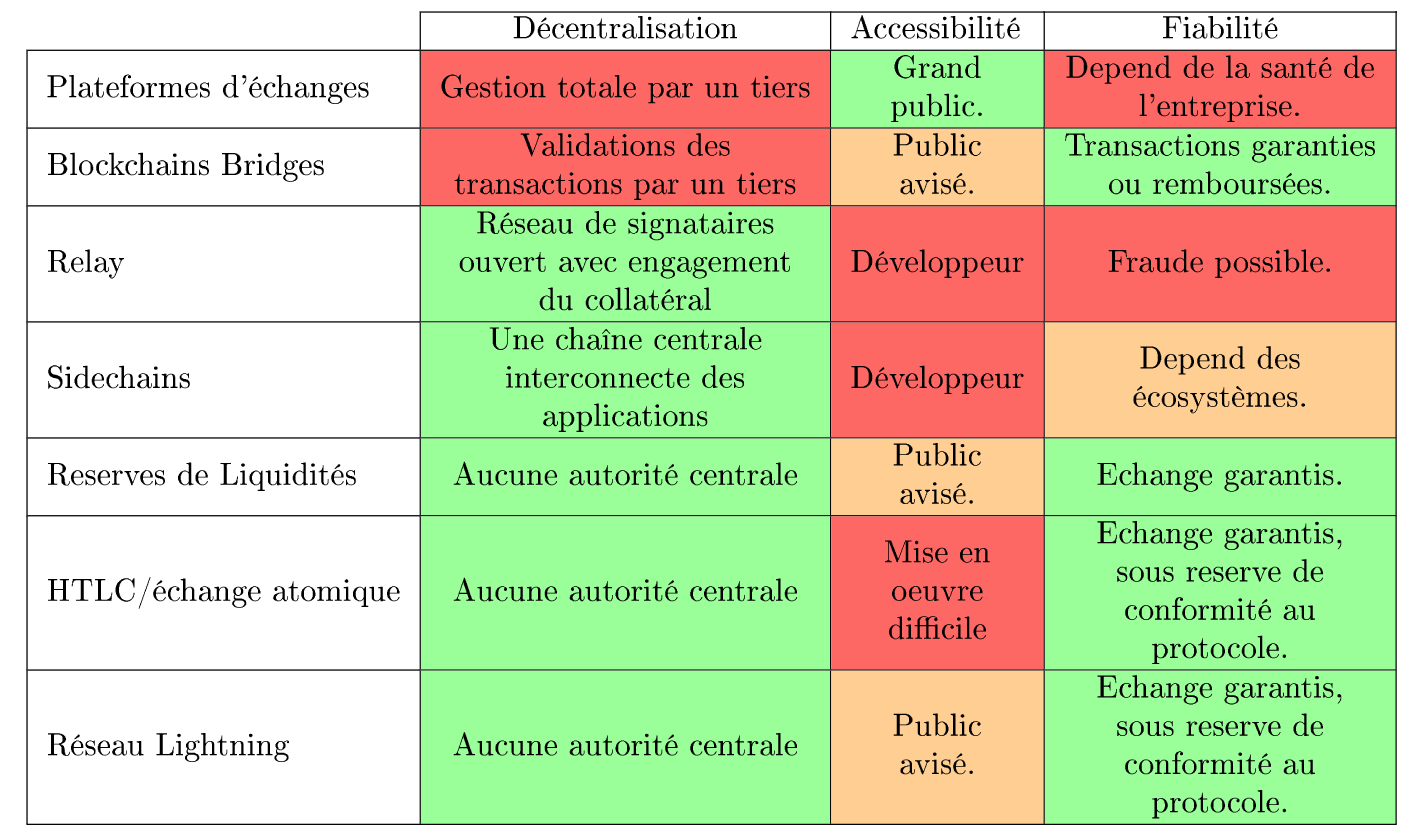
\includegraphics[scale = 0.2]{conclusion/tableau.png}
            \label{fig:recap}
            \caption{Tableau récapitulatif}
        \end{figure}
    \end{figure}
    
\end{frame}

\newpage
\section{Systèmes Décentralisés}
\begin{frame}{Centralisé}
    \begin{block}{Le centralisé offre\dots}
        \begin{itemize}
            \item Diversité d'acteurs.
            \item Accessibilité.
            \item Multiples fonctionnalités.
        \end{itemize}
    \end{block}
    \pause
    \begin{block}{Mais\dots}
        \begin{itemize}
            \item Opacité des protocoles.
            \item Failles de sécurité.
            \item Collecte des données.
        \end{itemize}
    \end{block}
\end{frame}


\begin{frame}{Décentralisé}
    \begin{block}{Le décentralisé offre\dots\dots}
        \begin{itemize}
            \item Pas de tiers de confiance.
            \item Transparence.
            \item Fiabilité accrue.
        \end{itemize}
    \end{block}
    \pause
    \begin{block}{Mais\dots}
        \begin{itemize}
            \item Difficiles d'accès.
            \item Intérêt économique faible.
        \end{itemize}
    \end{block}
\end{frame}

\begin{frame}{Conclusion générale}
    \begin{itemize}
        \item Flou entre centralisé/décentralisé.
        \item Définition variable.
    \end{itemize}
\end{frame}

\begin{frame}
    \begin{figure}
        \begin{figure}
            \centering
            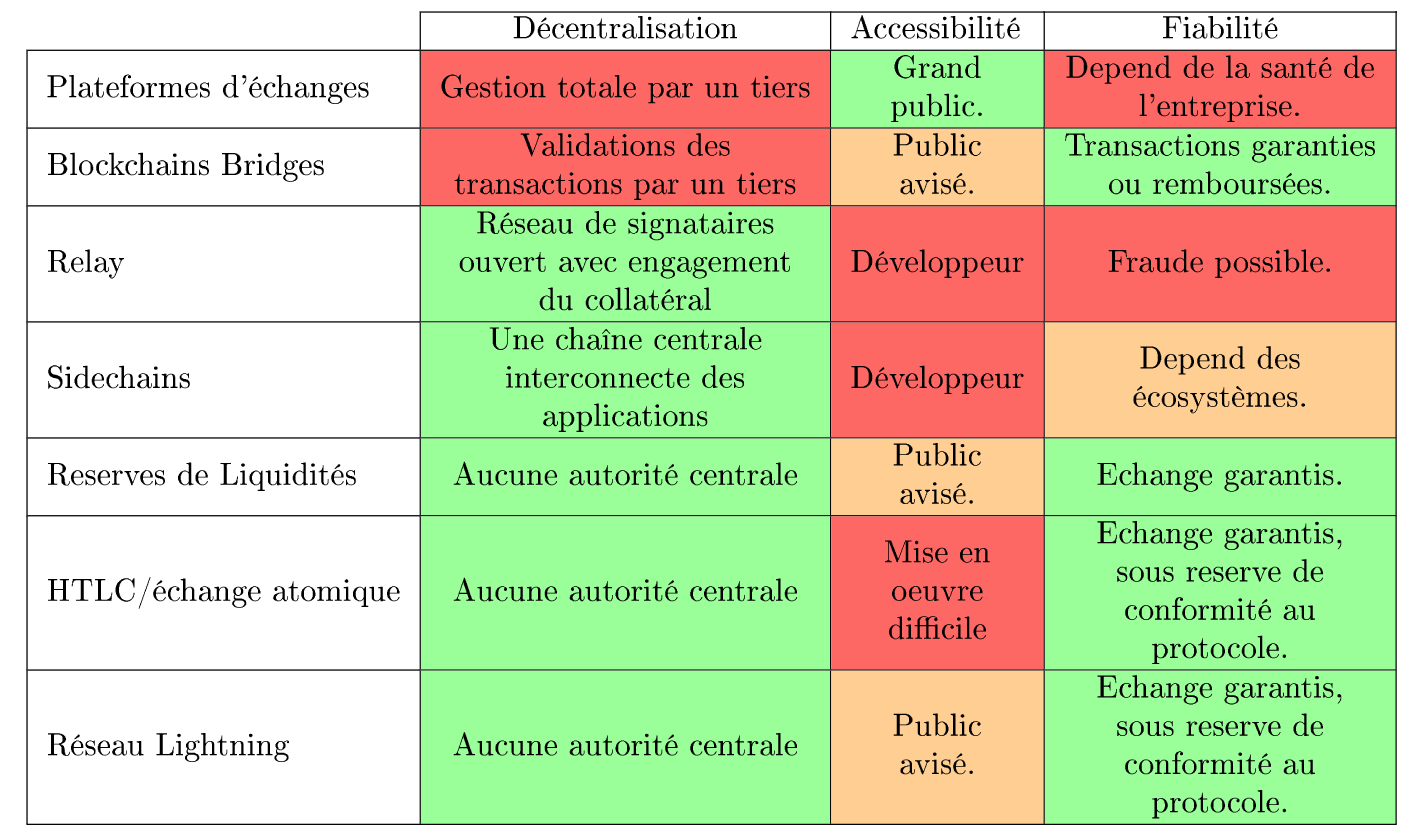
\includegraphics[scale = 0.2]{conclusion/tableau.png}
            \label{fig:recap}
            \caption{Tableau récapitulatif}
        \end{figure}
    \end{figure}
    
\end{frame}

\newpage
\printbibliography

\end{document}